\documentclass[12pt]{article}
\usepackage{fullpage,enumitem,amsmath,amssymb,graphicx}
\usepackage{graphicx} % This is a package for including graphics in your solution.
\usepackage{listings}
\usepackage[final]{pdfpages}

\begin{document}

\begin{center}
{\Large CS168 Spring Assignment 6}

\begin{tabular}{rl}
SUNet ID(s): 05794739 & \\
Name(s): & Luis A. Perez \\
Collaborators: &
\end{tabular}
\end{center}

By turning in this assignment, I agree by the Stanford honor code and declare
that all of this is my own work.

\section*{Part 1}

\begin{enumerate}[label=(\alph*)]
  \item We present the Laplacian matrix for each of the figures in turn.

    \begin{enumerate}[label=(\alph*)]
      \item
        This matrix consists of $1, 2, 2, \cdots, 2, 2, 1$ ($D$) along the diagonal, with $-1$s surrounding the main diagonal for $i = j + 1$ and $i = j - 1$ ($-A$).
        \[
          L = \begin{bmatrix}
            1 & -1 & 0 & 0 & \cdots & 0 & 0 & 0 & 0 \\
            -1 & 2 & -1 & 0 & \cdots & 0 & 0 & 0 & 0 \\
            0 & -1 & 2 & -1 & \cdots & 0 & 0 & 0 & 0 \\
            0 & 0 & -1 & 2 & \cdots & 0 & 0 & 0 & 0 \\
              &   &   &   & \vdots &   &   &   &   \\
            0 & 0 & 0 & 0 & \cdots & 0 & 0 & 0 & 0  \\
            0 & 0 & 0 & 0 & \cdots & -1 & 0 & 0 & 0  \\
            0 & 0 & 0 & 0 & \cdots & 2 & -1 & 0 & 0  \\
            0 & 0 & 0 & 0 & \cdots & -1 & 2 & -1 & 0  \\
            0 & 0 & 0 & 0 & \cdots & 0 & -1 & 2 & -1  \\
            0 & 0 & 0 & 0 & \cdots & 0 & 0 & -1 & 1
          \end{bmatrix}
        \]
      \item
        This is the same matrix as above, except the final row and column, which both consists entirely, and the diagonal. Nodes $1$ and $n-1$ now have degree $2$ while $n$ has degree $n-1$ and all other have degree $3$.

        \[
          L = \begin{bmatrix}
            2 & -1 & 0 & 0 & \cdots & 0 & 0 & 0 & -1 \\
            -1 & 3 & -1 & 0 & \cdots & 0 & 0 & 0 & -1 \\
            0 & -1 & 3 & -1 & \cdots & 0 & 0 & 0 & -1 \\
            0 & 0 & -1 & 3 & \cdots & 0 & 0 & 0 & -1 \\
              &   &   &   & \vdots &   &   &   &   \\
            0 & 0 & 0 & 0 & \cdots & 0 & 0 & 0 & -1  \\
            0 & 0 & 0 & 0 & \cdots & -1 & 0 & 0 & -1  \\
            0 & 0 & 0 & 0 & \cdots & 3 & -1 & 0 & -1  \\
            0 & 0 & 0 & 0 & \cdots & -1 & 3 & -1 & -1  \\
            0 & 0 & 0 & 0 & \cdots & 0 & -1 & 2 & -1  \\
            -1 & -1 & -1 & -1 & \cdots & -1 & -1 & -1 & n-1  \\
          \end{bmatrix}
        \]
      \item
        This matrix is exactly the same as that in (a), except the top-right and bottom-left corners also have a $-1$ entry and every entry in the diagonal is $2$.
        \[
          L = \begin{bmatrix}
            2 & -1 & 0 & 0 & \cdots & 0 & 0 & 0 & -1 \\
            -1 & 2 & -1 & 0 & \cdots & 0 & 0 & 0 & 0 \\
            0 & -1 & 2 & -1 & \cdots & 0 & 0 & 0 & 0 \\
            0 & 0 & -1 & 2 & \cdots & 0 & 0 & 0 & 0 \\
              &   &   &   & \vdots &   &   &   &   \\
            0 & 0 & 0 & 0 & \cdots & 0 & 0 & 0 & 0  \\
            0 & 0 & 0 & 0 & \cdots & -1 & 0 & 0 & 0  \\
            0 & 0 & 0 & 0 & \cdots & 2 & -1 & 0 & 0  \\
            0 & 0 & 0 & 0 & \cdots & -1 & 2 & -1 & 0  \\
            0 & 0 & 0 & 0 & \cdots & 0 & -1 & 2 & -1  \\
            -1 & 0 & 0 & 0 & \cdots & 0 & 0 & -1 & 2  \\
          \end{bmatrix}
        \]
      \item
        This matrix is the same as in (b) except for the fact that every diagonal entry except for $L_{nn}$ is $3$, $L_{n-1,1} = L_{1, n-1} = -1$.
        \[
          L = \begin{bmatrix}
            3 & -1 & 0 & 0 & \cdots & 0 & 0 & -1 & -1 \\
            -1 & 3 & -1 & 0 & \cdots & 0 & 0 & 0 & -1 \\
            0 & -1 & 3 & -1 & \cdots & 0 & 0 & 0 & -1 \\
            0 & 0 & -1 & 3 & \cdots & 0 & 0 & 0 & -1 \\
              &   &   &   & \vdots &   &   &   &   \\
            0 & 0 & 0 & 0 & \cdots & 0 & 0 & 0 & -1  \\
            0 & 0 & 0 & 0 & \cdots & -1 & 0 & 0 & -1  \\
            0 & 0 & 0 & 0 & \cdots & 3 & -1 & 0 & -1  \\
            0 & 0 & 0 & 0 & \cdots & -1 & 3 & -1 & -1  \\
            -1 & 0 & 0 & 0 & \cdots & 0 & -1 & 3 & -1  \\
            -1 & -1 & -1 & -1 & \cdots & -1 & -1 & -1 & n-1  \\
          \end{bmatrix}
        \]
    \end{enumerate}
  \item
    We plot the 8 requested figures. Please see Figure \ref{fig:line_graph}, Figure \ref{fig:line_graph_plus_one}, Figure \ref{fig:circle_graph} and Figure \ref{fig:circle_graph_plus_one}.

    These eigenvectors make perfect sense. The smaller eigenvectors are attempting to minimize the distances between neighbors in the graph, leading to smooth curves for the line and circle graphs since simply placing the points in order will decrease their neighbors distance. For the circle and line graphs with an additional point, similar curves are visible with the restriction that the $n$-th point is placed at $0$, since this is the closest to all other points.

    For the larger eigenvectors, we can see that they attempt to position neighbors as far away as possible. For the line graph, this gives rise to shapes where the closer to an endpoint a node is, the less distance it needs to be from its neighbors (because it's not connected to the other point). For the circle graph, we see that odd nodes are placed at one extreme, and even nodes at the other. When we include the additional node, we observe straight-forward behavior where the main goal is to separate that single node as much as possible from all the others.


      \begin{figure}[!ht]
        \centering
        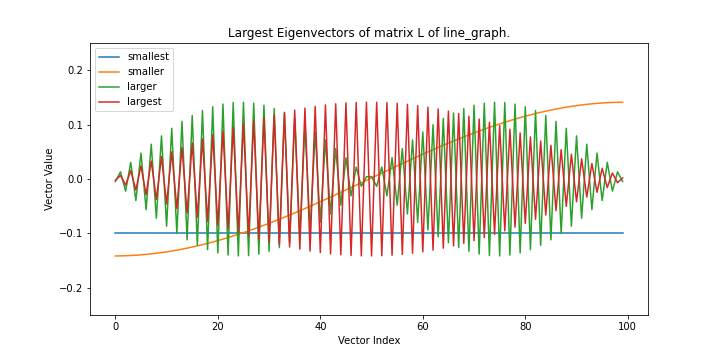
\includegraphics[scale=0.3]{figures/eigenvectors_line_graph_L.png}
        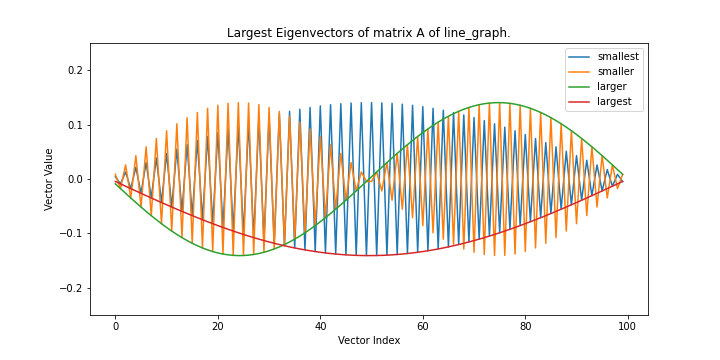
\includegraphics[scale=0.3]{figures/eigenvectors_line_graph_A.png}
        \caption{Eigenvectors for the laplacian and adjacency of the $n$-point line-graph. Vectors corresponding to the two smallest eigenvalues and vectors corresponding to the two largeest eigenvalues are shown for each case.}
        \label{fig:line_graph}
      \end{figure}

      \begin{figure}[!ht]
        \centering
        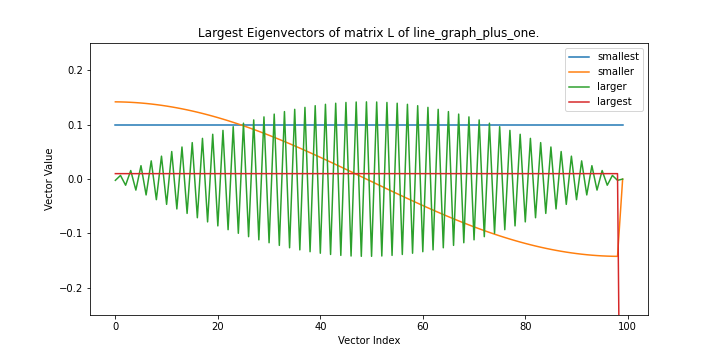
\includegraphics[scale=0.3]{figures/eigenvectors_line_graph_plus_one_L.png}
        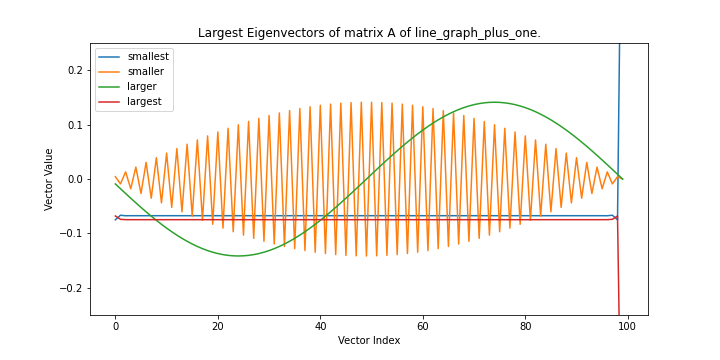
\includegraphics[scale=0.3]{figures/eigenvectors_line_graph_plus_one_A.png}
        \caption{Eigenvectors for the laplacian and adjacency of the $n-1$-point line-graph with a final point connected to all previous points. Vectors corresponding to the two smallest eigenvalues and vectors corresponding to the two largeest eigenvalues are shown for each case.}
        \label{fig:line_graph_plus_one}
      \end{figure}

      \begin{figure}[!ht]
        \centering
        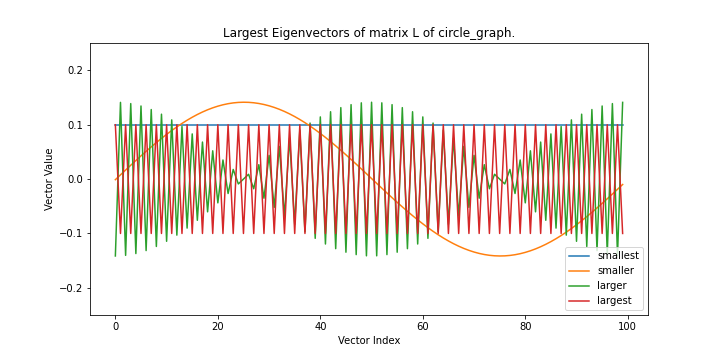
\includegraphics[scale=0.3]{figures/eigenvectors_circle_graph_L.png}
        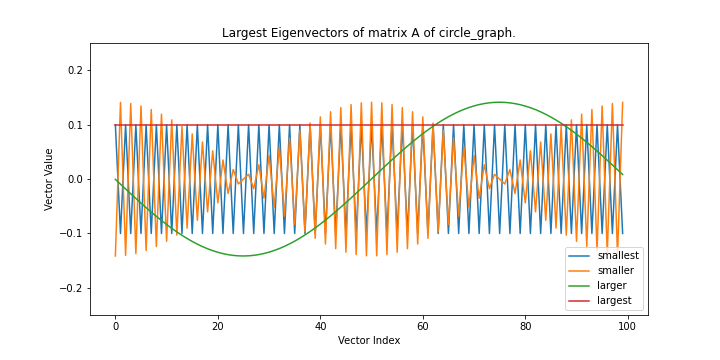
\includegraphics[scale=0.3]{figures/eigenvectors_circle_graph_A.png}
        \caption{Eigenvectors for the laplacian and adjacency of the $n$-point circle-graph. Vectors corresponding to the two smallest eigenvalues and vectors corresponding to the two largeest eigenvalues are shown for each case.}
        \label{fig:circle_graph}
      \end{figure}

      \begin{figure}[!ht]
        \centering
        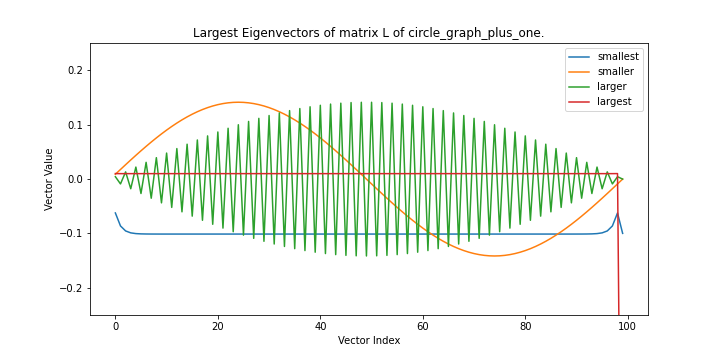
\includegraphics[scale=0.3]{figures/eigenvectors_circle_graph_plus_one_L.png}
        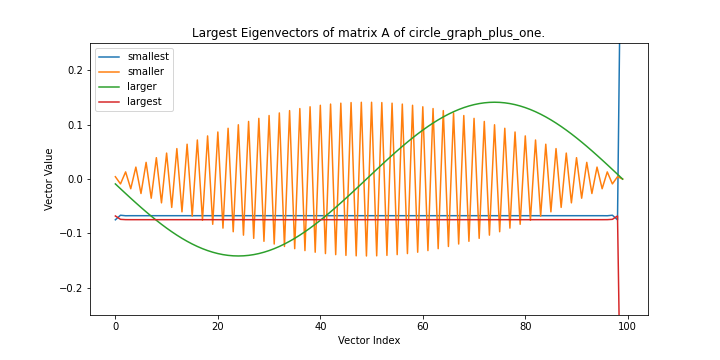
\includegraphics[scale=0.3]{figures/eigenvectors_circle_graph_plus_one_A.png}
        \caption{Eigenvectors for the laplacian and adjacency of the $n-1$-point circle-graph with a final point connected to all previous points. Vectors corresponding to the two smallest eigenvalues and vectors corresponding to the two largeest eigenvalues are shown for each case.}
        \label{fig:circle_graph_plus_one}
      \end{figure}

    \item
      See Figure \ref{fig:projections} for the plots of the four graphs embedded onto the 2nd and 3rd smallest eignevalues.

      \begin{figure}[!ht]
        \centering
        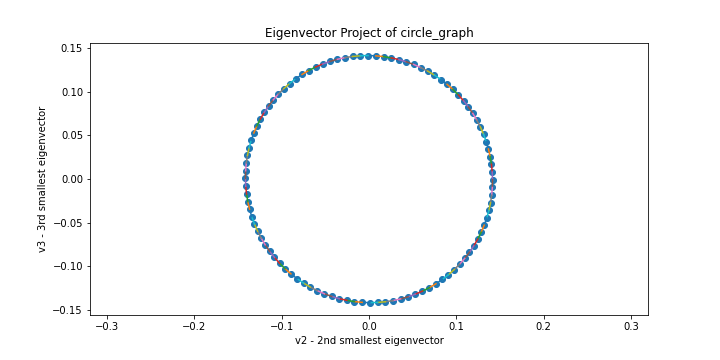
\includegraphics[scale=0.3]{figures/eignevector_projection_circle_graph.png}
        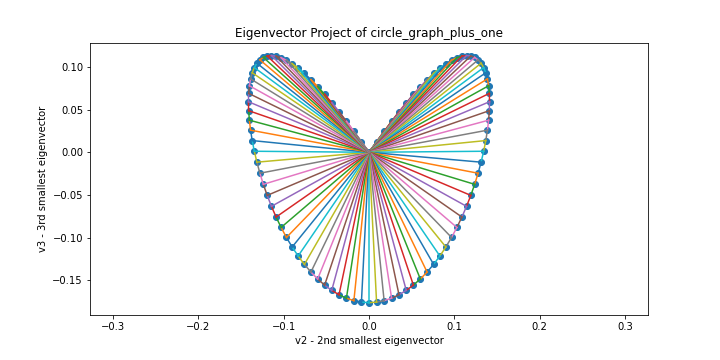
\includegraphics[scale=0.3]{figures/eignevector_projection_circle_graph_plus_one.png}
        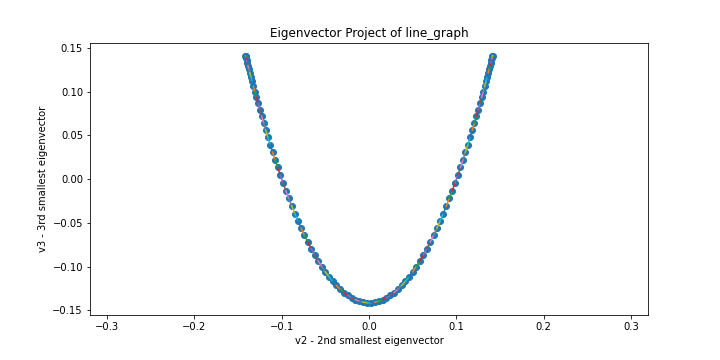
\includegraphics[scale=0.3]{figures/eignevector_projection_line_graph.png}
        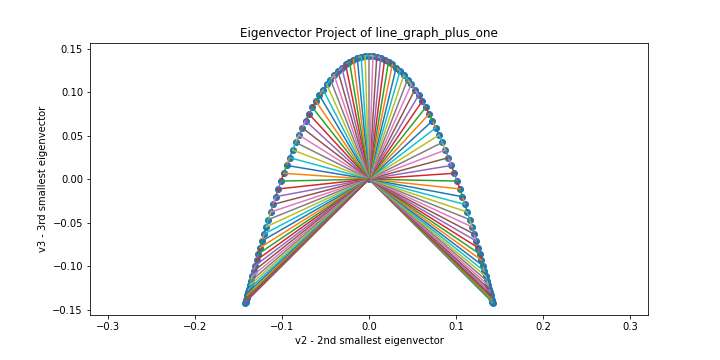
\includegraphics[scale=0.3]{figures/eignevector_projection_line_graph_plus_one.png}
        \caption{Projections of different types of graphs onto their second and third smallest eigenvectors.}
        \label{fig:projections}
      \end{figure}

    \item 
      The requested plot can be seen in Figure \ref{fig:random_projection}. We note that the points whose x and y coordinates are less than $\frac{1}{2}$ are clustered together. The reason this makes sense is because the smaller eighvectors are trying to minimize the $L_2$ distance between neighbors. Since we defined the graph to form and edge between two nodes whose $L_2$ distance was less than $\frac{1}{4}$, it is immediately clear that all points in the lower left quadrant (whose x and y coordinates are less than $\frac{1}{2}$) will be connected (the distance between them, by definition, will be less than $\frac{1}{4}$). As such, in the projection, these points will tend to cluster so as to minimize their distance since they are neighbors in the graph.

      \begin{figure}[!ht]
        \centering
        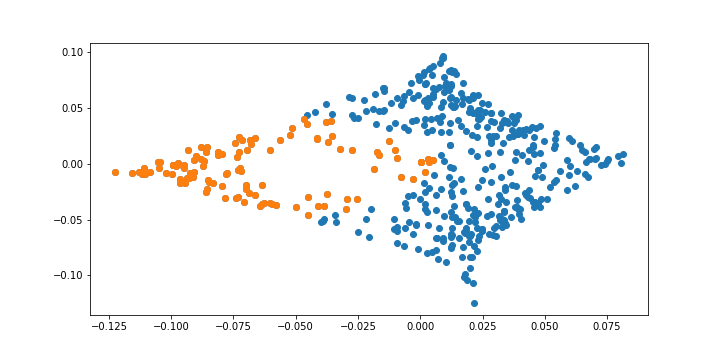
\includegraphics[scale=0.5]{figures/cluster_random.png}
        \label{Projection onto second and third smallest eigenvectors of random graph where connectivity is defined by L2 distance less than 0.25.}
        \label{fig:random_projection}
      \end{figure}

\end{enumerate}

\section*{Part 2}

\begin{enumerate}[label=(\alph*)]
  \item See Appendix.
  \item
    Smallest 12 eigenvalues, in order:
    \begin{verbatim}
      0.000
      0.000
      0.000
      0.000
      0.000
      0.000
      0.014
      0.054
      0.074
      0.081
      0.120
      0.133
    \end{verbatim}
  \item
    Given the results from (b), it appears that the graph has 6 connected components, since the multiplicity of the $0$ eigenvalue of the Laplacian is $6$. This follows from Theorem 2.1 in Lecture 11.

    The sizes of the largest and second largest components are 1,484 and 3 respectively. We found this by finding 6 clusters in the eigenvectors. We repeated for a few eigenvectors to confirm.

  \item 
    We now report the three disjoint low conductance sets. We found all three sets using the $9$-th smallest eigenvector, which we plot in Figure \ref{fig:9th_smallest}. We first searched for a small set (of size between $150$ and $300$ that satisfied the conductance requirement by looking at points which were all within some $t$ units of $0$). Once we identified this set, the other $2$ were found using the same eigenvector through a sliding window approach, where we looked for points which were shifted up or down from the previous set by some fixed amount.

    We describe this process for each set in more detail below.

    \begin{itemize}
      \item $S_1$. This set comes from the $9$-th smallest eigenvector, see Figure \ref{fig:9th_smallest}. It contains $229$ elements and has a conducatance of $~0.0887$. $10$ members are:
      \begin{verbatim}
         2,    6,  519,    8,  521,  522, 1032, 1036,   13,  527
      \end{verbatim}
      This set was found by identifying the vertices whose values in the 9th eigenvector were in the range $0 \pm 0.0002$.
      \item $S_2$. This set comes from the $9$-th smallest eigenvector, see Figure \ref{fig:9th_smallest}. It contains $561$ elements and has a conducatance of $~0.0586$. $10$ members are:
      \begin{verbatim}
         1,  3,  4,  9, 10, 11, 14, 16, 19, 20
      \end{verbatim}
      This set was found by identifying the vertices whose values in the 9th eigenvector were in the range $0.00235 \pm 0.00215$.

      \item $S_3$. This set comes from the $9$-th smallest eigenvector, see Figure \ref{fig:9th_smallest}. It contains $362$ elements and has a conducatance of $~0.0867$. $10$ members are:
      \begin{verbatim}
          5,  7, 23, 27, 30, 42, 44, 46, 47, 50
      \end{verbatim}
      This set was found by identifying the vertices whose values in the 9th eigenvector were in the range $0.00469 \pm 0.00019$.
    \end{itemize}
    \begin{figure}[!ht]
      \centering
      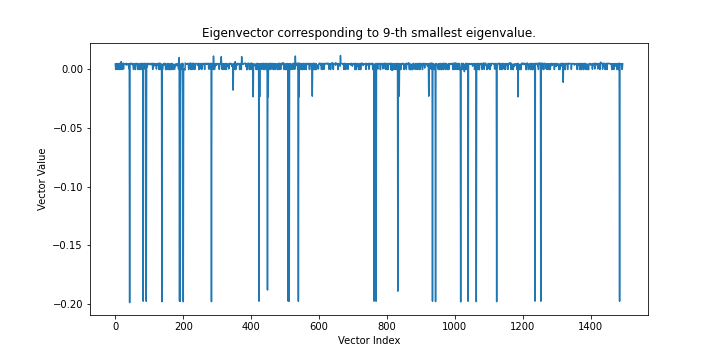
\includegraphics[scale=0.5]{figures/eigenvector_9.png}
      \caption{Eigenvector corresponding to 9th smallest eigenvalue - used to identify low conductance clusters.}
      \label{fig:9th_smallest}
    
    \end{figure}
  \item The conductance of the randomly selected set of 150 nodes is 0.9085. This seems to indicate that the overall graph structure is not very tight (conductance is high for a random subgraph). As such, the groups identified above appear to be very tightly knit communities with little interaction outside their groups.
\end{enumerate}


\newpage
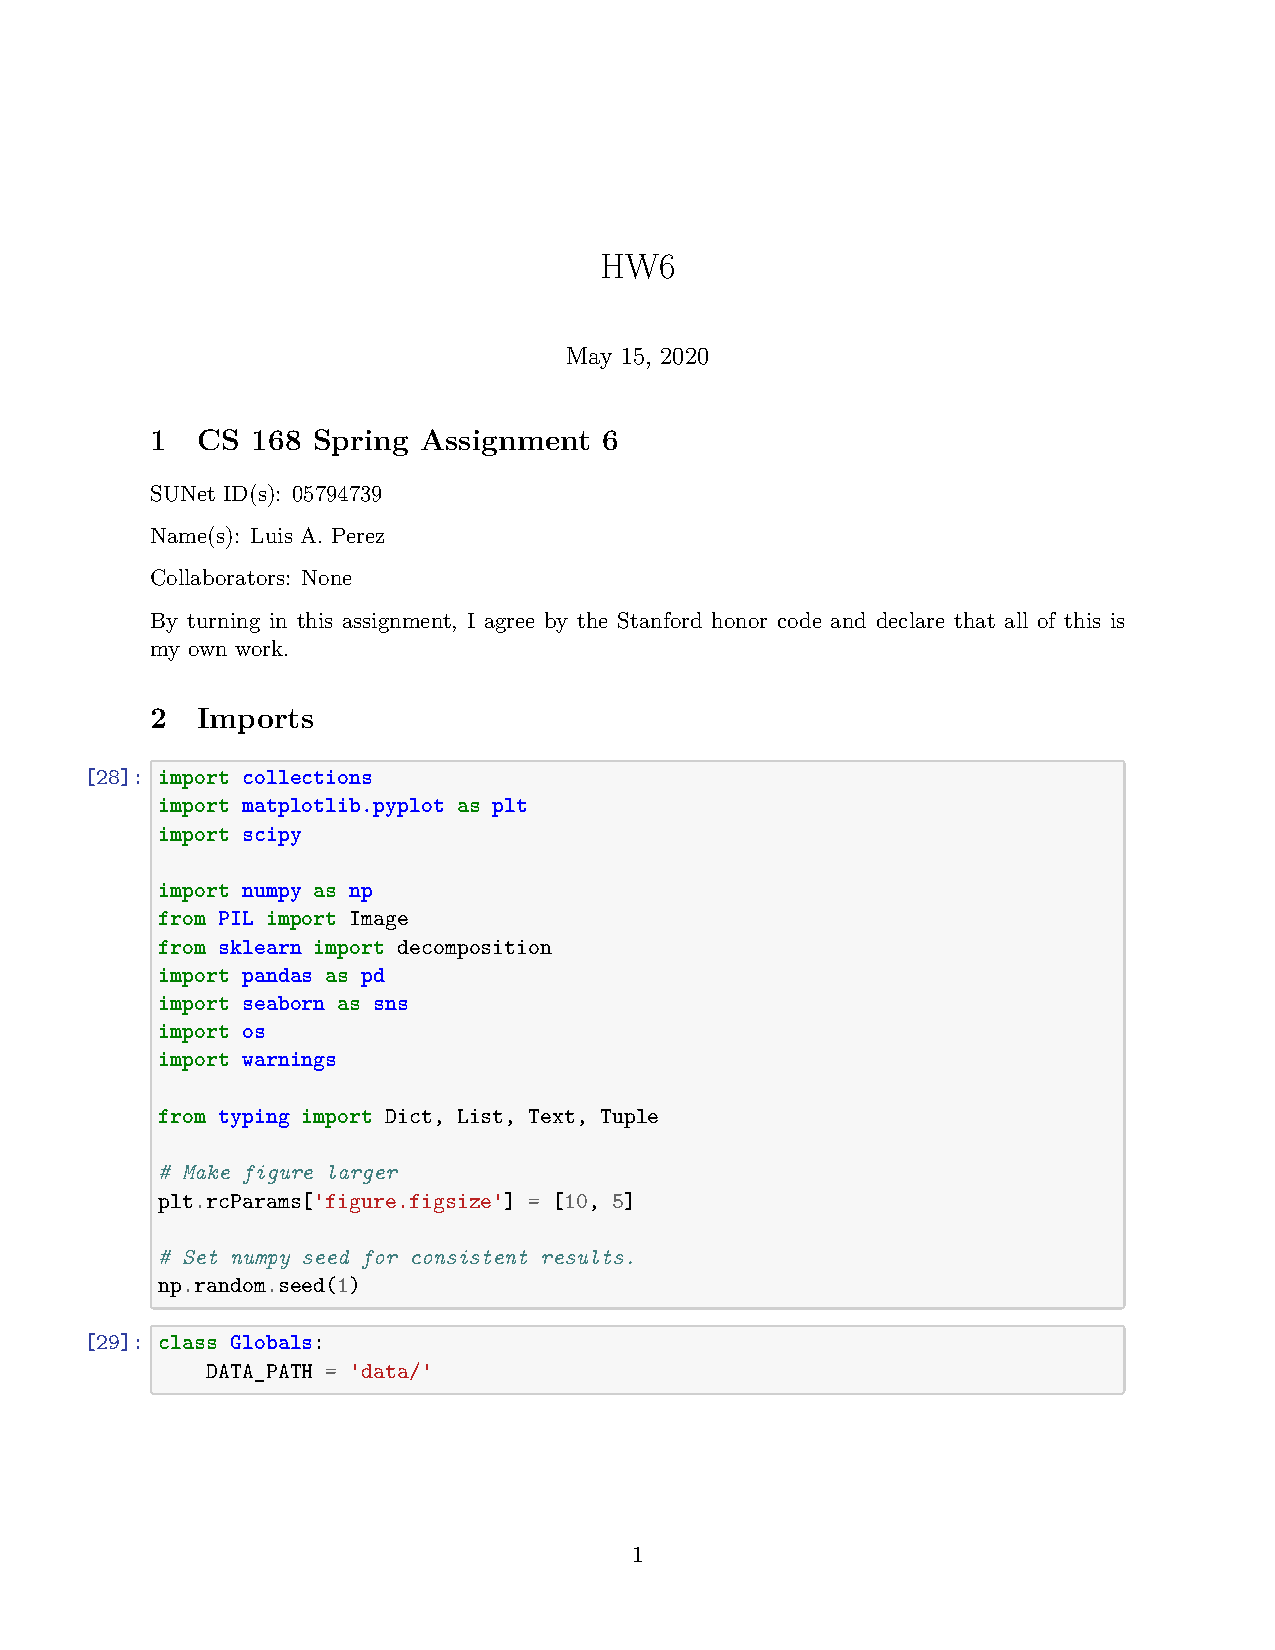
\includepdf[pages=-]{HW6}

\end{document}
